\documentclass{article}

\usepackage{full page}  % make the margins somewhat smaller than the default
\usepackage{graphicx}    % needed for including graphics e.g. EPS, PS
\usepackage{hyperref}     % needed for hyperlink
\usepackage[]{algorithm2e}
\usepackage{mathtools}
\usepackage{listings}  % needed for source code listings
\lstset{language=Java}         

% set the document title, author, and date here.
%  once set, the \maketitle command (within the document)
%  will display them nicely
\title{Sphere Sampling in CSpace for Motion Planning}
\author{Yinan Zhang}

\begin{document}
\maketitle

\section{Introduction}

Traditionally, sampling based motion methods use discrete data to construct paths for motion tasks. The disadvantage of this kind of implementation is obvious: 

\begin{enumerate}
  \item CSpace is a continuous space, discrete samples cannot represent it well;
  \item Many samples are actually not necessary and consume a lot of memory, e.t. samples far away from obstacles.
  \item The way to get optimal path using samples in the free space requires building a dense roadmap, like PRM*.
\end{enumerate}

Our method is to sample spheres which contain collision-free area in configuration space. Using these hyper-spheres in c-space, we can:
\begin{enumerate}
  \item describe configuration space in a continuous way;
  \item find an optimal path;
  \item save memory by reducing unnecessary samples.
\end{enumerate}

\section{Sphere Sampling Algorithm}
\label{Sphere sampling algorithm}
 \begin{algorithm}
 	\KwData{Configuration Space}
 	\KwResult{Spheres that cover most of the free space}
 	s0 = sampleSphere( randomly position );\\
 	S = \{s0\}; \\
 	\tcp{Every two boundary points distance equals to $\delta$}
 	boundaryQueue = a queue that contains all boundary points of s0;\\
 	\While{ boundaryQueue is not empty }{
 		\tcp{Candidate point to sample next sphere.}
 		point = boundaryQueue.pop(); \\
 		\If{ point not in any spheres } {
 			si = sampleSphere( point );\\
 			\If{ $\delta$ $\leq$ si.radius } {
 				S = S $\cap$ \{si\}; \\
 				boundaryQueue.put( all boundary points of si ); 
 			}
 		}
 	}
 	\caption{ Sphere sampling algorithm }
 \end{algorithm}

	\subsection{Something we know}
    \subsubsection{How to interpret the algorithm? }
      Our algorithm can be viewed as a combination of RRT and visibility-PRM. In each iteration of our algorithm, we get some more spheres center at the edge of existing ones, it rapidly and randomly grows until converge. Unlike RRT, these spheres build not only a tree rooted at the starting sphere, if we build the overlapping relationship of them, each sphere can also be viewed as a node of a roadmap. In a visibility PRM algorithm, if we limit the range a sample can view to a certain distance, or the distance from itself to the nearest obstacle, we can get pretty much the same result, which is why I view these spheres as a visibility roadmap. Inside each sphere, a robot is free to go anywhere without worrying about collision. 

		\subsubsection{Will the algorithm stop?}
 			\label{Finite number of spheres}
 			As is shown in the algorithm, we get boundary points of an existing sphere by limiting the distance between every two points to be equal to $\delta$. Then the algorithm samples new spheres centered at these points. So the distance between two spheres centers is always larger than or equal to $\delta$. 

 			The problem is equivalant to proof there could be finite number of points put in the space such that the distance between every two points is larger than or equal to $\delta$.

 			Assume we partition the whole configuration space( including free space and obstacle space ) into hyper-cubes. The length of every edge of these hyper-cubes is exactly $\delta$. As long as the configuration space has finite volume, the number of hyper-cubes is finite. Assume the number of hyper-cubes is N, the number of hyper-cubes that is totall or partly in free space is less than N. Thus the number of spheres is finite, and less than N.

 			So the algorithm will always converge.	

 		\subsubsection{$\delta$-clearance}
 			\cite{Karaman2011} proposed an algorithm, named PRM*, to find a path. It requires the actual optimal path to have $\delta$-clearance so the algorithm can find a approximately optimal path. Yet, the algorithm cannot explicitly control the quality of the path by defining $\delta$. In our alogrithm, we can define the actually value of $\delta$ and control the coverage of free-space by sampling spheres. 

 		\subsubsection{Find Containing Spheres}
 			In the algorithm, we need to know if a candidate point is inside any spheres. Naively, we need to iterate each existing spheres to determine if a point is inside, which requires O(n) time. This can fortunately be done with less time by hashing spheres to uniform grids of the c-space. Each grid contains references to spheres that intersect/contain the grid. By hasing a candidate point in the same way, we can easily know if a point is inside any spheres already.

 			(Can we use Locally Sensitive Hashing?)  

 		\subsubsection{Inaccurate matric}
			Suppose we have an inccurate matric which gives us the distance to obstacle:
 			dist[i] = accurate\_dist[i]/c[i], where 1 $\leq$ c[i] $\leq$ upper\_bound. When sampling at a point near the obstacle, dist[i] = accurate\_dist[i]/c[i] = $\delta$ the algorithm will stop sampling at that point. So the farthest distance from spheres boundary to obstacles is $\delta$ * upper\_bound. 

 			If the optimal path has $\delta$ * upper\_bound clearance. The algorithm can still cover the path and eventually find it.

    \subsubsection{How to fast determine if there exist a path between two configurations?}
      One thing I like particularly about this methods is that it can fast determine if there exist a feasible path between two configurations. Usually in PRM* which builds a very dense roadmap, if we want to know whether there exists a path or not, we should run the A* search on the graph, by iterating all nodes in the graph, A* search will finally tell you it failed. It this case, A* search requires exponential time because it has to iterate all nodes in very depth of the graph. 

      However, if we view the problem as finding a chain of spheres that contains start and goal configurations at the head and end of the chain, it will cost much less time to search the roadmap built by overlapping spheres. Because the number of spheres will be much less than the number of samples in a dense roadmap, and the number of edges is way less than a dense roadmap, which means even in the worst case, an exponential runtime will be much less than that required by A* searching a dense graph. 
   
    \subsubsection{Does the shape of C-Space matter? }
      I think the answer is clearly a YES. For example, the C-Space for a two-joint robot arm is donut-shaped. However, I represent it in a square-shaped space by connecting the ends of X and Y axis to the heads of them. 

      Also, if the moving range of two joints are not both [0, 2$\pi$], say one is [0, $\pi$/100], the space would look like a really narrow rectangle. However, I still recommend scalling the space to a cube-like shape with equal length of both dimension. Because after sampling, if we scale the space back to what it was, spheres became ellipses, these ellipses covere more space than the same number of spheres. 

      Another benefit of transforming the space is we probably don't need to care about the matric in original C-Space, I simply use Euclidean distance. 

    \subsubsection{How to deal with unlinked parts of configuration space?}
      A C-space can be partitioned into several parts by obstacles, each part is not linked to others, and there is no path from one to another. 

      The proposed solution to this problem is exactly what visibility PRM will do. In v-PRM, coverage is measured by the number of attemps failed to get a new sample. For example, if we failed n times to get a new sample, the coverage of the visibility graph to the C-space is 1 - 1/n. Here, I think this method can also be used to solved our problem, given an acceptable failure times, say k, we try to randomly sample a configuration that is not in any sphere. If we successfully get a new sample within k attemps, run the sphere sampling algorithm again, then we can cover the isolated part of C-space. If we cannot get a new sample within k attemps, our spheres have covered 1 - 1/k of the c-space. 

    \subsubsection{What else can these spheres do?}
      Bialkowski uses similar spheres in his work \cite{Bialkowski2012} to help doing efficient collision detection.

      For multi-robot motion planning problem, this spheres, generated in a single robot's configuration space, can be reused for other robots. It saves a lot of time because, we don't need to sample in multi-robot configuration space. This is mentioned in \cite{Bialkowski2013} 

  \subsection{Demo}
    \begin{figure}[ht]
      \centering
      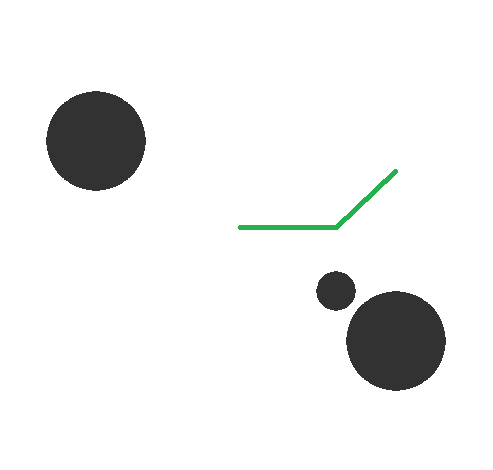
\includegraphics[width=4in]{PhysicSpace_Origin.PNG}
      \caption{Physics World}
      \label{fig:PhysicsWorld}
    \end{figure}

    Figure \ref{fig:PhysicsWorld} is the physics world a 2-joint robot arm is in. Black circles are obstacles. The robot arm cannot move in X or Y axis, but can rotate two joints in range [0, 2$\pi$]

    \begin{figure}[ht]
      \centering
      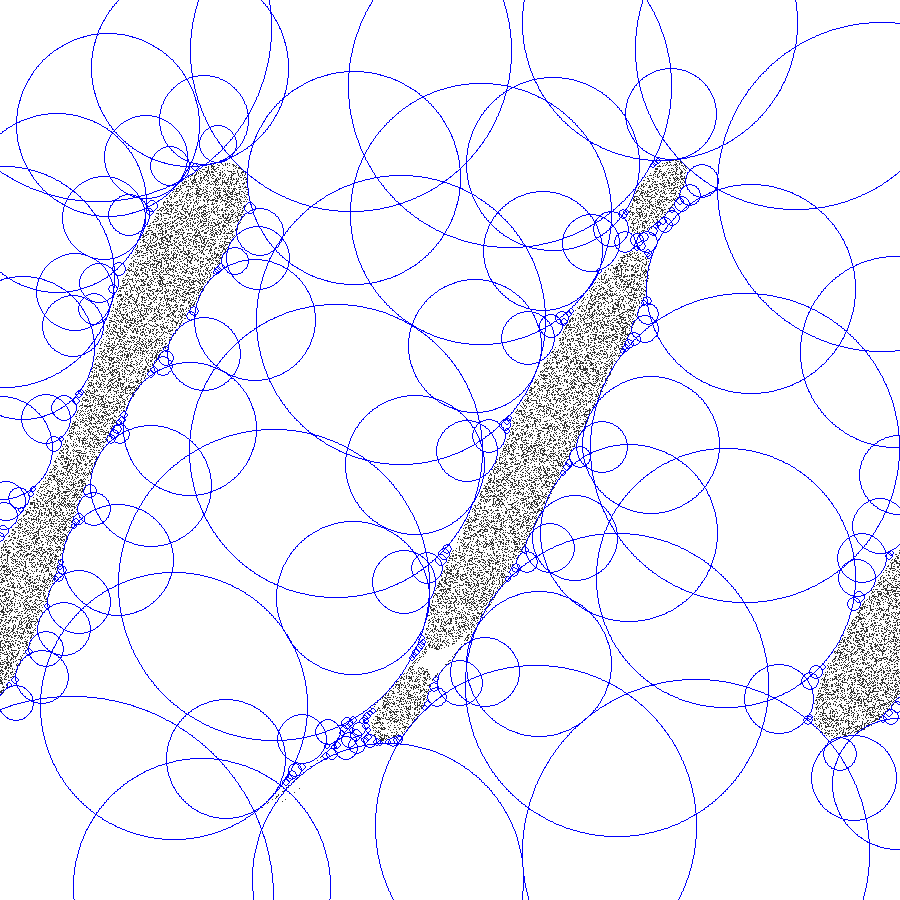
\includegraphics[width=4in]{CSpace.PNG}
      \caption{C-Space covered by spheres}
      \label{fig:C-Space}
    \end{figure}

    The figure \ref{fig:C-Space} shows the corresponding configuration space of the robot arm. (NOTE: This is actually a torus-shaped space. ) Spheres you can see are sampled by our method.

	\subsection{Some Questions:}
 		\subsubsection{How to use less hyper-spheres to cover the space?}
    As can be seen in Figure \ref{fig:C-Space}, in some places there are many annoying small spheres. If these small spheres can be covered by some bigger spheres without breaking the property of containing only free-space, it can save more memory.  

 		\subsubsection{How to get the distance to obstacles more accurately?}
    For now, we shoot several rays from a configuration to all directions in C-Space, then return the shortest distance to obstacles. This is actually not a very good idea, but since everybody else is using it. I didn't hesitate to use it. However, this is not good, actually, it still uses discrete data to represent continuous space. This method is not accurate. If there is a better way to know the distance to nearest obstacles, it would be great.

\section{Path search search}
  We use A* search to find the path.

  \label{Path searching algorithm}
  \begin{algorithm}[H]
  \KwData{spheres, start configuration, goal configuration}
  \KwResult{a path that connects start and end configuratioin.(or fail)}
  openSet = priority queue containing start; \\
  closedSet = empty set; \\
  \While{ openSet is not empty }{
    current = remove lowest rank point from openSet; \\
    \If{ neighbor == goal }{
        backtrain( neighbor )
    }
    add current to closedSet; \\
    neighbors $\gets$ getSuccessors( current ); \\

    add current to closedSet;\\
    \ForEach{neighbor in neighbors}{
        cost $\gets$ g(current) + movementcost(current, neighbor); 

        \If{neighbor not in openSet or cost < g(neighbor)}{
          parent(neighbor) $\gets$ current;\\
          g(neighbor) $\gets$ cost;\\
          heuristic $\gets$ movementcost( neighbor, goal );\\
          F $\gets$ heuristic + cost;\\
          openSet.push( neighbor, F );\\
        }
    }
  }
  \caption{ Search a path }
  \end{algorithm}


 \begin{algorithm}
  \KwData{point, goal}
  \KwResult{successor points}
  sphere = get the sphere that contains point; \\
  \eIf{ sphere contains goal }{
    return goal.
  }{
    return boundary points of sphere, less than $\delta$ distance away.
  }
 \caption{ getSuccessors()\label{IR} }
 \end{algorithm}
 
  \subsection{Something we know}
    \subsubsection{How to reduce unnessary neighbors}
      In the method we simpling get all boundary points of a sphere with less than $\delta$ distance to each other. Actually, about half of them are not necessary legal neighbors. Some points belong to the sphere their parent is from, these points are useless, because if a path leaves a sphere then enter the same sphere again, it is surely not an optimal path. Giving up these points will save memory as well as run time about 50\%. 


  \subsection{Something we don't}
    \subsubsection{How to estimate the quality of the path?}
      I don't know how to make sure the algorithm finds the optimal path. This is something I wrote last time:

        "Assuming the path maintains $\delta$ clearance, the worst path found by our algorithm is this: the optimal path is in a chain of spheres with radius $\delta$. The point our algorithm chooses to use is $\delta$ / 2 away from the actual point the path is going through.Then the chosen path is 2 times of length of the actual optimal path. "

      One thing I can think of is post processing. After getting a path, we can determine if we can connect every other or more points in the path directly, thus avoids redundant distance. ( Triangular inequality ) 

    \subsubsection{A better to find the path?}
      A* search is fine, it finds good quality path. However, A* search still try to discretize information we get from sampling spheres, which is the reason why we get 2 times longer path in the worst case. A method I think probably will work is to solve an equation and find the point. The equation requires: 
      \begin{enumerate}
        \item The point is in the intersection of the line from its parent to its son and the sphere it belongs to.
        \item The new path is still totally inside the same sphere chain containing the original path. 
      \end{enumerate}
      
      This is equivalent to post processing, I guess. Do it several times until it converge, then the path should be optimal.

      Proof? Err.... Let me think about it....  

\section{Demo}
    \begin{figure}[h]
      \centering
      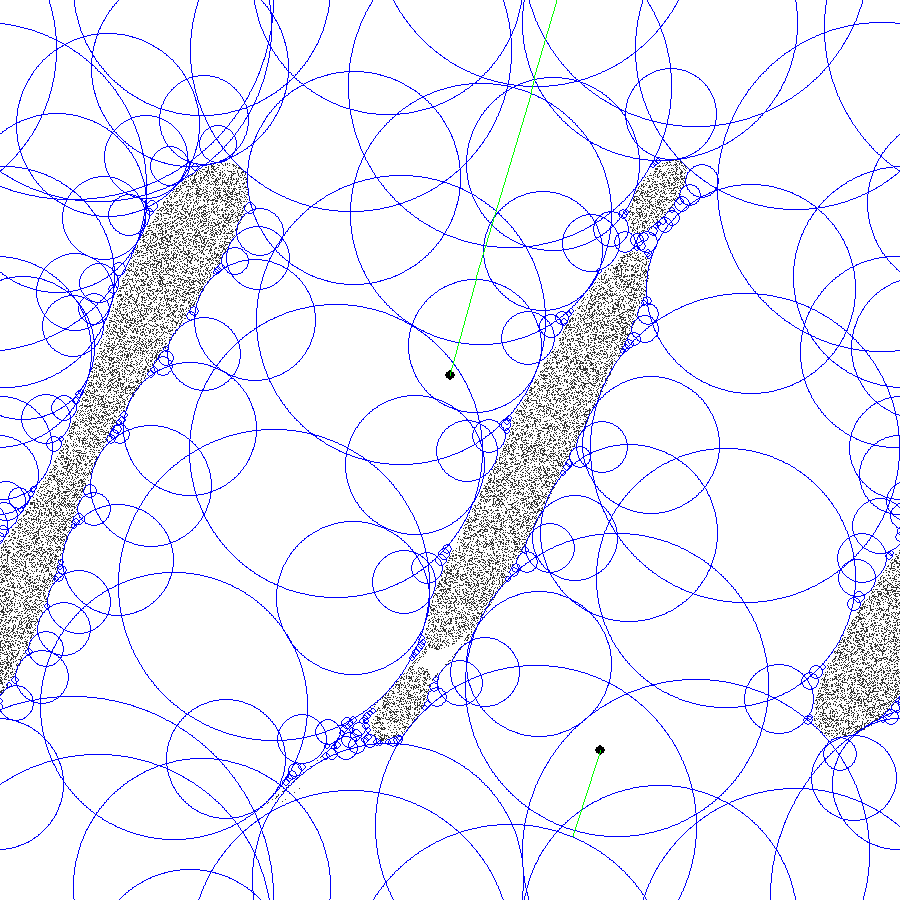
\includegraphics[width=4in]{Path1.PNG}
      \caption{Path finding problem 1}
      \label{fig:path1}
    \end{figure}
    \begin{figure}[h]
      \centering
      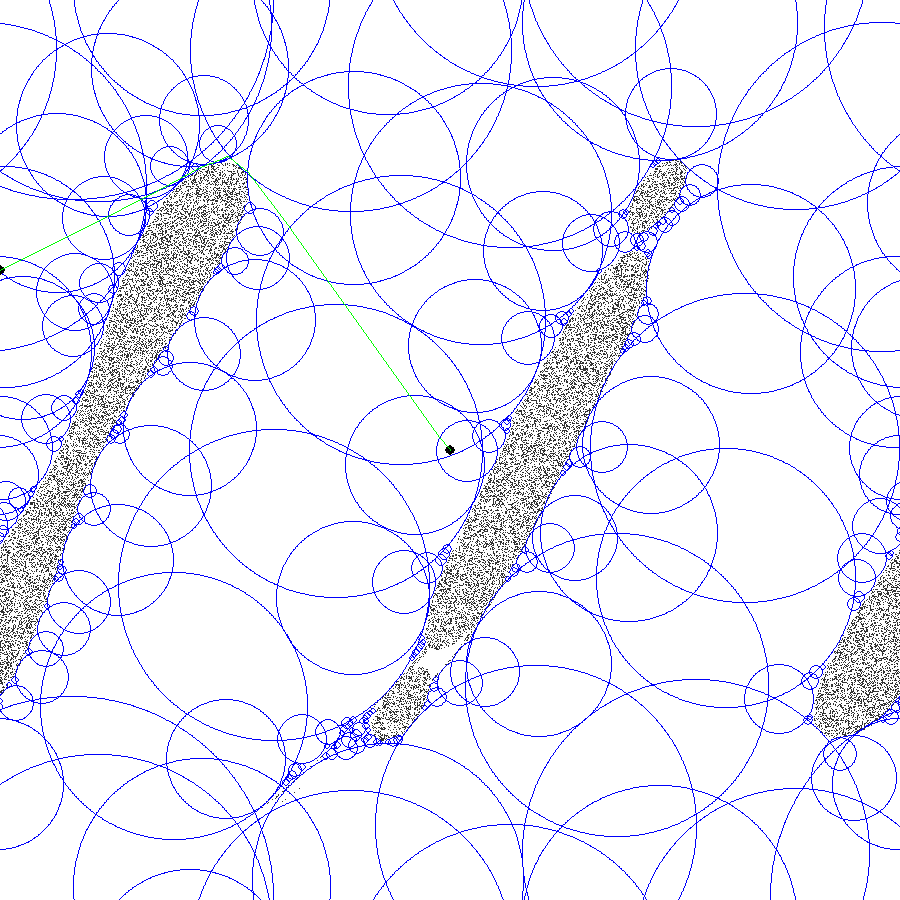
\includegraphics[width=4in]{Path2.PNG}
      \caption{Path finding problems 2}
      \label{fig:path2}
    \end{figure}

    Figure \ref{fig:path1} and Figure \ref{fig:path2} show two path finding problems solutions in scaled configuration space. Black dots are start and goal configurations. (Remember, the c-space is donut-shaped) Obviously, the path is approximately optiaml.

    Corresponding robot movements are shown in Figure \ref{fig:move1} and Figure \ref{fig:move2}:

    \begin{figure}[h]
      \centering
      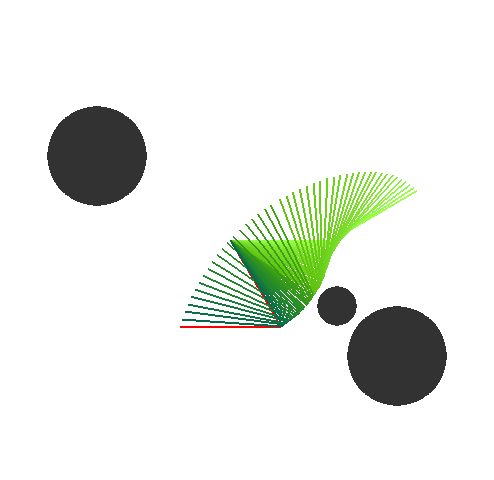
\includegraphics[width=4in]{Movement1.PNG}
      \caption{Robot Movement 1}
      \label{fig:move1}
    \end{figure}

    \begin{figure}[h]
      \centering
      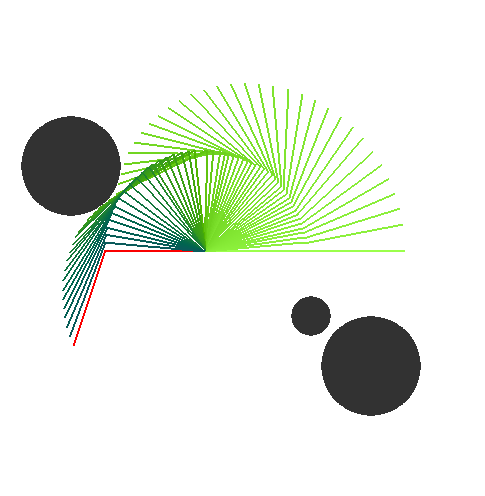
\includegraphics[width=4in]{Movement2.PNG}
      \caption{Robot Movement 2}
      \label{fig:move2}
    \end{figure}

    Video can be find in youtube: 
    
    \url{http://youtu.be/u7BlHCwnKNc}
    \href{http://youtu.be/u7BlHCwnKNc}{ Motion Planning solution 1 }

    \url{http://youtu.be/8IY8MltdVGI}
    \href{http://youtu.be/8IY8MltdVGI}{ Motion Planning solution 2 }

\section{Experiment}
  \subsection{ Num. of Spheres VS Obstacle area in C-Space }
    \begin{figure}[h]
      \centering
      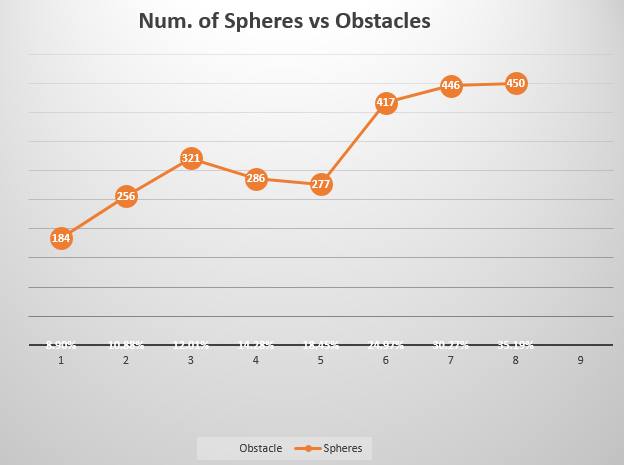
\includegraphics[width=4in]{Chart.PNG}
      \caption{Chart}
      \label{fig:chart1}
    \end{figure}
    
    In order to estimate the memory cost of the algorithm, we use the number of spheres as a criteria. Because spheres are the only data we need to reserve after running the algorithm. The number of spheres is a hint of memory cost of representing C-Space as a sphere-based roadmap. 

    Figure \ref{fig:chart1} shows the relationship between the number of spheres and the obstacle area in C-Space.

\begin{thebibliography}{9}

\bibitem{Karaman2011}
  Karaman, Sertac, and Emilio Frazzoli,
  \emph{"Sampling-based algorithms for optimal motion planning"}.
  The International Journal of Robotics Research 30.7 (2011): 846-894.

\bibitem{Bialkowski2012}
  Bialkowski, Joshua, et al.
  \emph{"Efficient collision checking in sampling-based motion planning."}. Algorithmic Foundations of Robotics X. Springer Berlin Heidelberg, 2013. 365-380.

\bibitem{Bialkowski2013}
  Bialkowski, Joshua, Michael Otte, and Emilio Frazzoli. 
  \emph{"Fast Collision Checking: From Single Robots to Multi-Robot Teams."}. 
  arXiv preprint arXiv:1305.2299 (2013).

\end{thebibliography}

\end{document}
